\chapter{\label{chap:chap3} Projeto}



A organização e a descrição deste projeto serão apresentados neste capítulo.
Para tal, nas seções a seguir abordaremos a arquitetura, o formato de mensagens, módulos e submódulos que o constituem.

\section { Arquitetura }

Seguindo a topologia da Figura \ref{fig:fig14}, podemos observar que os \textit{fog nodes} não possuem um nodo central como servidor.
Sendo assim, os fog nodes e os edge devices comunicam-se utilizando o protocolo CoAP.
Dessa maneira, as Requisições entre fog nodes só ocorre caso o nodo requisitante saiba, previamente, o endereço IP relativo ao nodo solicitado.

\begin{figure}[H]
    \centering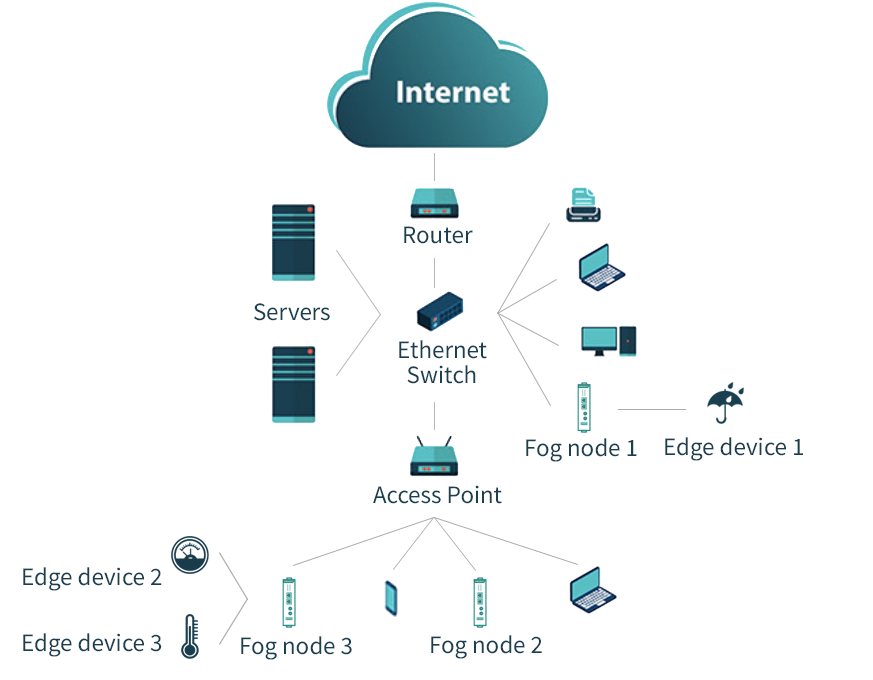
\includegraphics[width=.8\textwidth]{fig14.png}
    \caption [Topologia LAN]
    {\label{fig:fig14} Topologia LAN.}
\end{figure}

Em razão da topologia distribuída, a arquitetura deve ser capaz de mapear e sincronizar, de forma autônoma, os recursos providos pelos fog nodes.
Dessa forma, cada \textit{fog node} saberá quais são os \textit{edge devices} disponíveis na rede, portanto,
o nodo que possui o sensor de chuva saberia que existe um outro nodo em sua LAN capaz de medir a temperatura, por exemplo.

A arquitetura proposta, no que se refere a comunicação entre fog nodes e edge devices, utilizou como base um fork da implementação do protocolo CoAP\cite{coapimpl:2018}.
Esse fork, implementado em Python e de acordo com a RFC-7252, consiste em dois grandes módulos: \textit{CoAP-Server} e \textit{CoAP-Client}.
O primeiro, é responsável pelo recebimento das Requisições, e foi alterado com o objetivo de proporcionar o dinamismo na inserção e remoção dos recursos sem a necessidade de sua reinicialização.
O segundo módulo é encarregado de realizar as Requisições diretamente aos nodos, e para essa funcionalidade nenhuma alteração no projeto original foi realizada.


Observando a Figura \ref{fig:fig15}, podemos notar que a arquitetura de um fog node é composta por três grandes camadas, sendo elas hardware, sistema operacional e aplicações.

Na camada de hardware podemos utilizar desde um dispositivo com limitações de memória e CPU até um aparelho com grande capacidade computacional.
Já na camada de sistema operacional, temos a liberdade de utilizar uma vasta diversidade de distribuições Unix.
Por fim, na camada de aplicação devemos executar os processos \textit{CoAP-Server}, \textit{CoAP-Client} e \textit{Resource-Mapping}.

\begin{figure}[H]
    \centering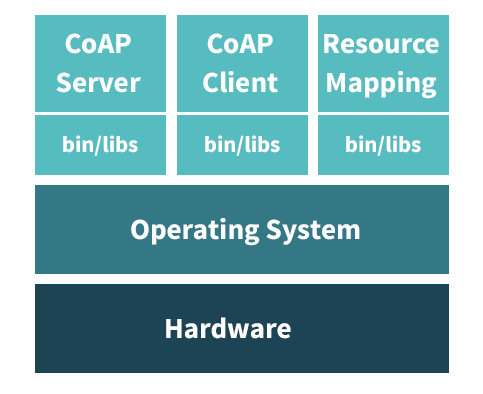
\includegraphics[width=.5\textwidth]{fig15.png}
    \caption[Arquitetura de um fog node]
    {\label{fig:fig15} Arquitetura de um fog node.}
\end{figure}

A Figura \ref{fig:fig16} exibe, de maneira detalhada, os processos envolvidos na execução no protocolo \textit{Resource-Mapping}.
Nela podemos destacar a presença de três entidades principais, \textit{Observer}, \textit{Keep Alive} e \textit{Receptor}.
Abaixo elencaremos as funcionalidades de cada entidade.

\begin{itemize}
    \item \textit{Observer} é responsável por manter o estado de seus proprios recursos atualizados.
    \item \textit{Keep Alive} tem a missão de manter seus vizinhos de rede atualizados sobre seu estado de operação.
    \item \textit{Receptor} é incumbido de receber e processar as requições recebidas via \textit{Resource-Mapping}.
\end{itemize}

\begin{figure}[H]
    \centering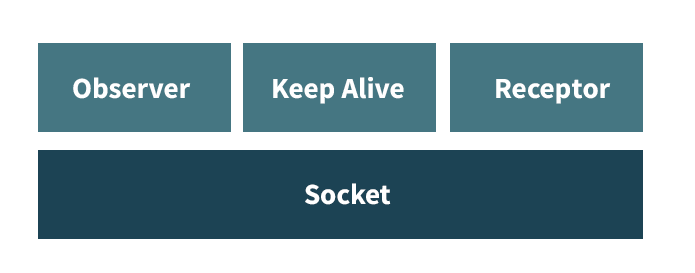
\includegraphics[width=.5\textwidth]{fig16.png}
    \caption[Arquitetura Resource-Mapping]
    {\label{fig:fig16} Arquitetura Resource-Mapping.}
\end{figure}


\section{Requisitos e limitações}

Para que a solução opere corretamente, tanto no mapeamento quanto na sincronização de recursos, algumas limitações e requisitos necessitam ser expostas.

Como proposição inicial temos que o sistema operacional deve ser Unix e o usuário corrente deve dispor de privilégios de root.
Além disso, a linguagem de programação Python em sua versão 2.7 com seu respectivo gerenciador de pacotes, \textit{PIP}\cite{pip}, devem estar instalados.
Por fim, os dados que os edge devices fornecerão aos fog nodes serão tratados de forma simulada, pois o funcionamento exato dos sensores e atuadores
fogem do escopo desse projeto. As Seções 4.3.1 e 4.3.2 utilizarão essas simulações a fim de validar o protocolo.


\section{Formato de mensagens}

Esta Seção define a pilha de protocolos a serem utilizados neste projeto, a justificativa pelas suas escolhas, e por fim, o detalhamento do protocolo proposto.
A pilha de protocolos atuará em conjunto com a organização arquitetural previamente definida na Figura \ref{fig:fig1}.

A fim de facilitar a compreensão da arquitetura deste projeto, a Figura \ref{fig:fig2} explicita a pilha de protocolos que o projeto fará uso para implementar as funcionalidades propostas.

\begin{figure}[htb!]
    \centering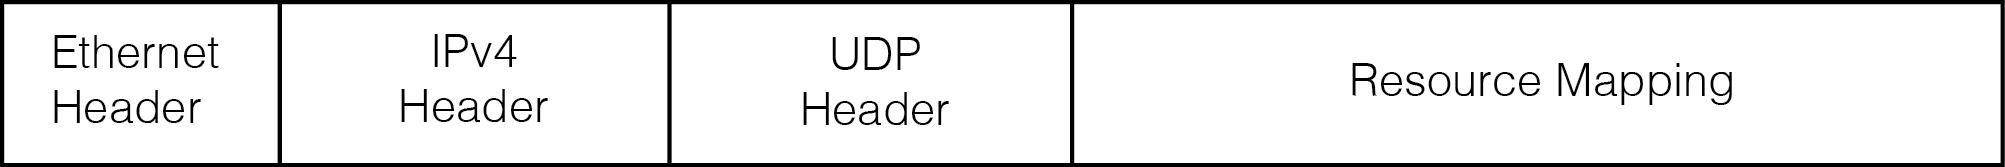
\includegraphics[width=.8\textwidth]{fig2.png}
    \caption[Pilha de protocolos]
    {\label{fig:fig2} Pilha de protocolos.}
\end{figure}

O modelo de referência TCP/IP é constituido de cinco camadas: física, enlace, rede, transporte e aplicação \cite{tanenbaum2011redes}.
Nesse trabalho, o níveis de rede e transporte (IPv4 e UDP respectivamente) serão utilizados para a implementação do modelo proposto.

A utilização de IPv4 na camada de rede justifica-se pelo fato do protocolo ser empregado em redes locais, que geralmente não necessitam de uma quantidade de endereçamento tão grande 
se comparado ao IPv6, mas não existem impedimentos para que implementações futuras utilizem IPv6 na camada de rede.

Manter o contexto de conexão entre os nodos, utilizando TCP por exemplo, despenderia uma quantidade de trafego desnecessário na rede.
Visto que o baixo custo na transmissão de dados é um dos objetivos desse trabalho, a utilização de datagramas UDP faz sentido para que a se aumente o desempenho da solução.

A Figura \ref{fig:fig12} apresenta, de forma detalhada, a estrutura dos dados contidos no protocolo \textit{Resource Mapping}.

\begin{figure}[htb!]
    \centering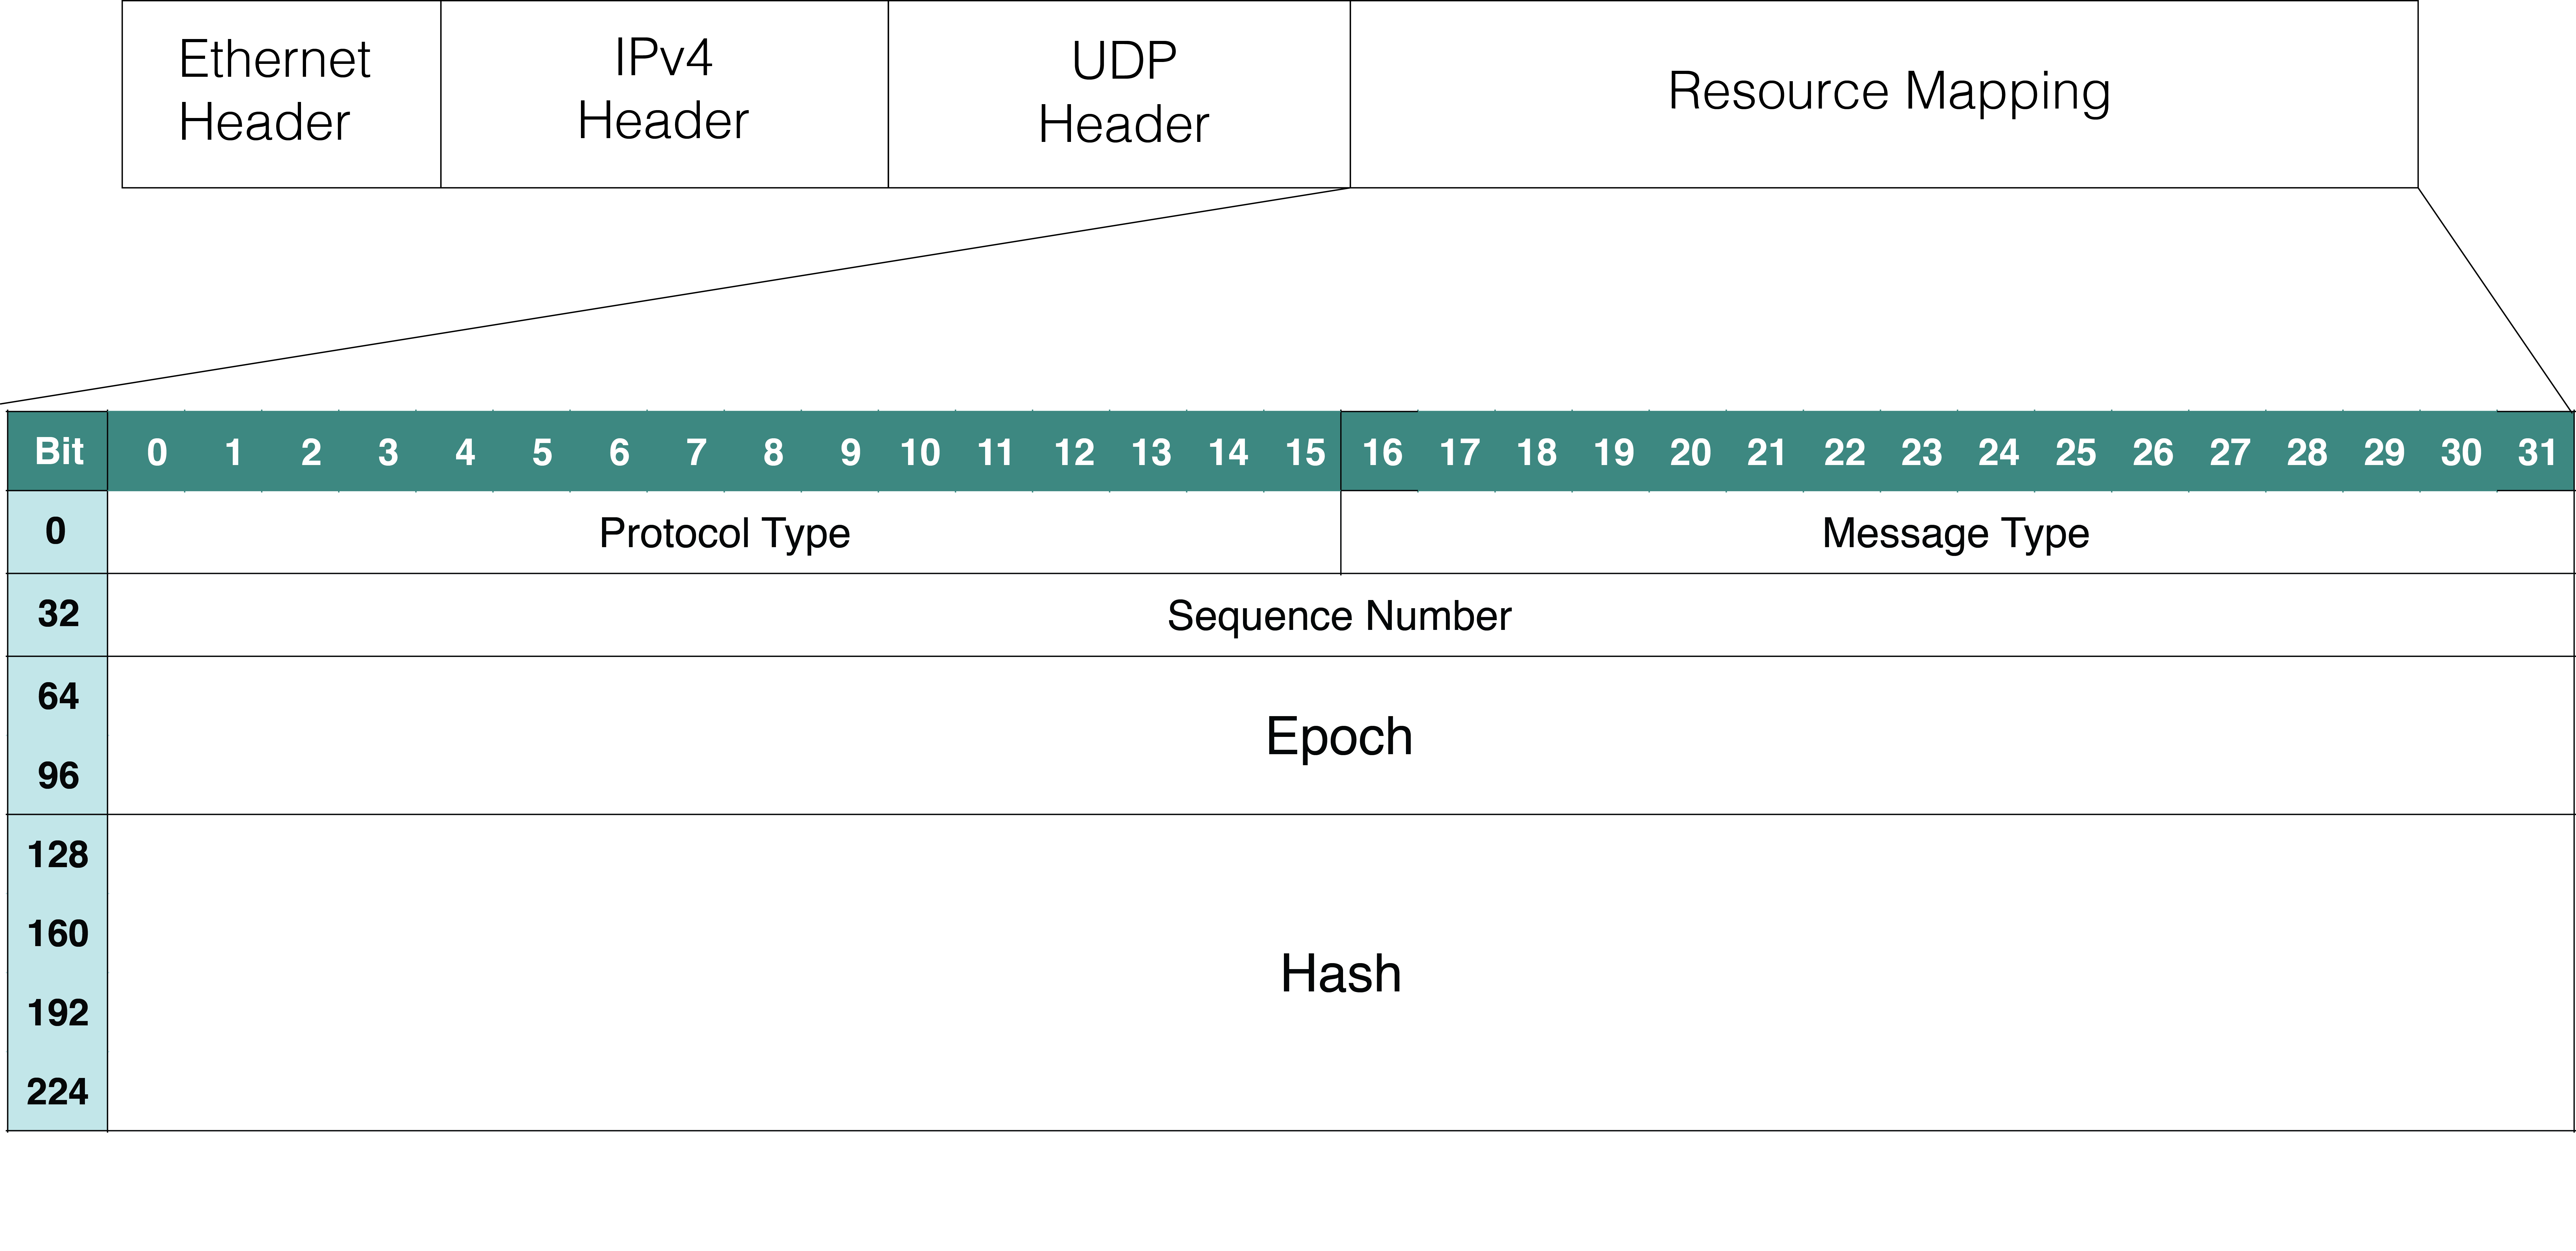
\includegraphics[width=.8\textwidth]{fig12.png}
    \caption[Detalhamento Resource Mapping]
    {\label{fig:fig12} Detalhamento Resource Mapping.}
\end{figure}

\begin{itemize}
\item O campo Protocol Type é reservado para indicar a forma de encapsulamento do pacote.
Dessa forma, o restante dos campos do pacote podem ser tratados de acordo com a definição dada pelo campo.
\item Atualmente existem dois tipos de Messages Types possíveis, keep alive e acknowledgement.
\item Sequence Number tem o intuito de identificar o pacote enviado.
\item O campo Epoch é utilizado para indicar alterações nos recursos providos pelo fog node.
Sendo assim, quando um recurso é adicionado ou removido de um fog node, o campo Epoch é acrescido em uma unidade. Os detalhes de seu comportamento serão abordados na Seção 3.3.2.
\item O campo Hash utiliza a função de criptografia MD5 para validar a integridade dos demais campos contidos no pacote.
\end{itemize}

O protocolo proposto, intitulado \textit{Resource Mapping}, como apresentado nas Figuras \ref{fig:fig2} e \ref{fig:fig12}, atuará na camada de aplicação do modelo de referência TCP/IP \cite{tanenbaum2011redes} e será responsável por padronizar, descobrir e sincronizar os nodos da névoa.
Os maiores desafios neste modelo proposto são manter o estado global dos recursos acessível a todos os nodos, e garantir que o desempenho seja satisfatório com o objetivo permitir a escalabilidade da solução.


\section{Módulos}

De forma geral, cada nodo da rede mantém uma lista com os endereços IP`s que fazem parte do mapeamento.
Atrelado à cada endereço IP,  há uma lista com os recursos providos por este.
Em vista disso, cada nodo contém um mapeamento global de recursos disponíveis na névoa.

O detalhamento das funcionalides que o projeto possui, tal como ilustrações relacionadas aos fluxos, serão abordadas nas proximas subseções.

\subsection{Descoberta de recursos}


Partindo do pressuposto que os nodos da névoa já possuem seus recursos devidamente criados e acessíveis via CoAP,
como primeiro passo do mapeamento devemos considerar a entrada de um novo nodo na rede.
No momento em que o nodo dispor de um endereço IP válido, este deverá enviar um pacote para o endereço de multicast indicando que possui recursos a serem disponibilizados.


Ao receberem o pacote enviado por multicast, os nodos que desejarem saber quais recursos estão sendo providos por este novo membro, deverão realizar uma Requisição
unicast para a URI \textit{/.well-known/core} utilizando o protocolo CoAP.
Vale lembrar que este fluxo de requisição e resposta, utilizando a URI \textit{/.well-known/core}, faz com que o nodo requisitado retorne todos seus recursos ao solicitante.

\begin{figure}[H]
    \centering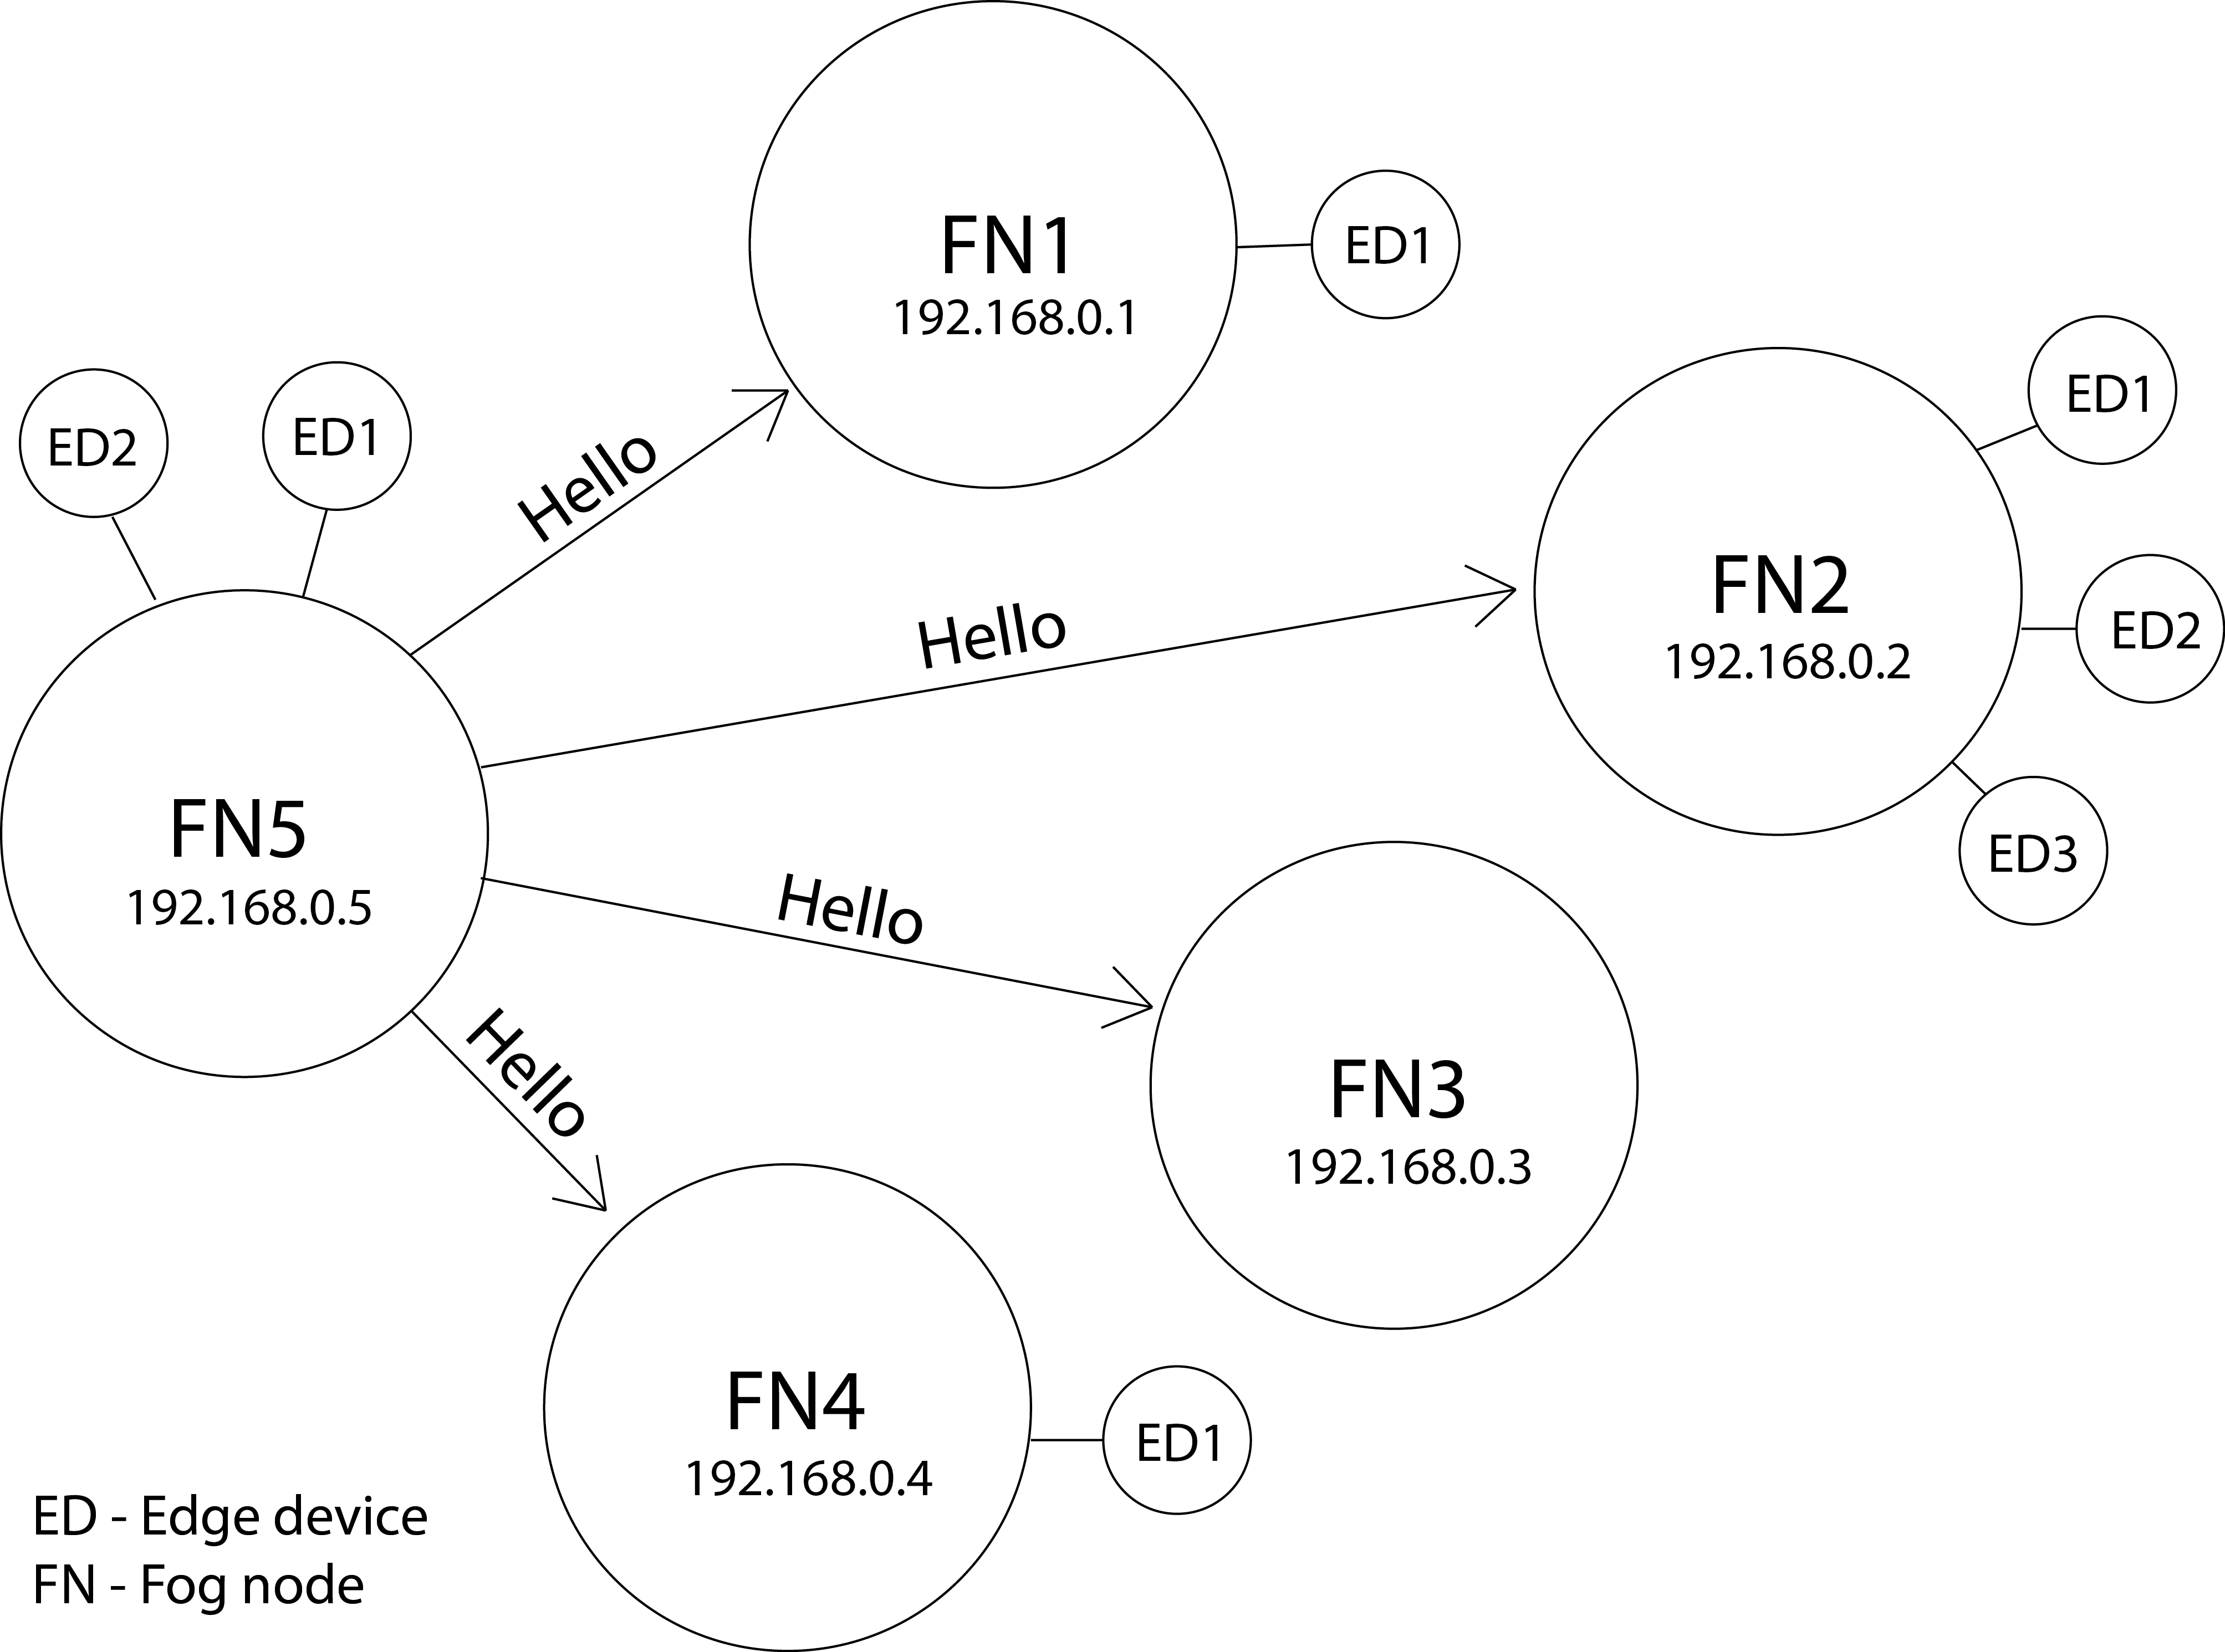
\includegraphics[width=.8\textwidth]{fig5.png}
    \caption[Nodo entrando na névoa]
    {\label{fig:fig5} Nodo entrando na névoa.}
\end{figure}

A topologia da névoa utilizada nas Figuras \ref{fig:fig5} e \ref{fig:fig6} é definida por fog nodes enumerados de um a cinco, sendo o nodo FN5 o último a entrar na rede.
A figura \ref{fig:fig5} demonstra o nodo FN5 entrando na névoa e, portanto, deverá anunciar-se por multicast indicando que possui recursos a serem disponibilizados.

Após FN5 enviar mensagem de Olá por multicast, os nodos FN1, FN2 e FN4 realizam a Requisição CoAP diretamente ao FN5 afim de obter os recursos disponíbilizados por ele,
já o nodo FN3, por não estar executando o protocolo de mapeamento, não realiza a Requisição CoAP.

\begin{figure}[H]
    \centering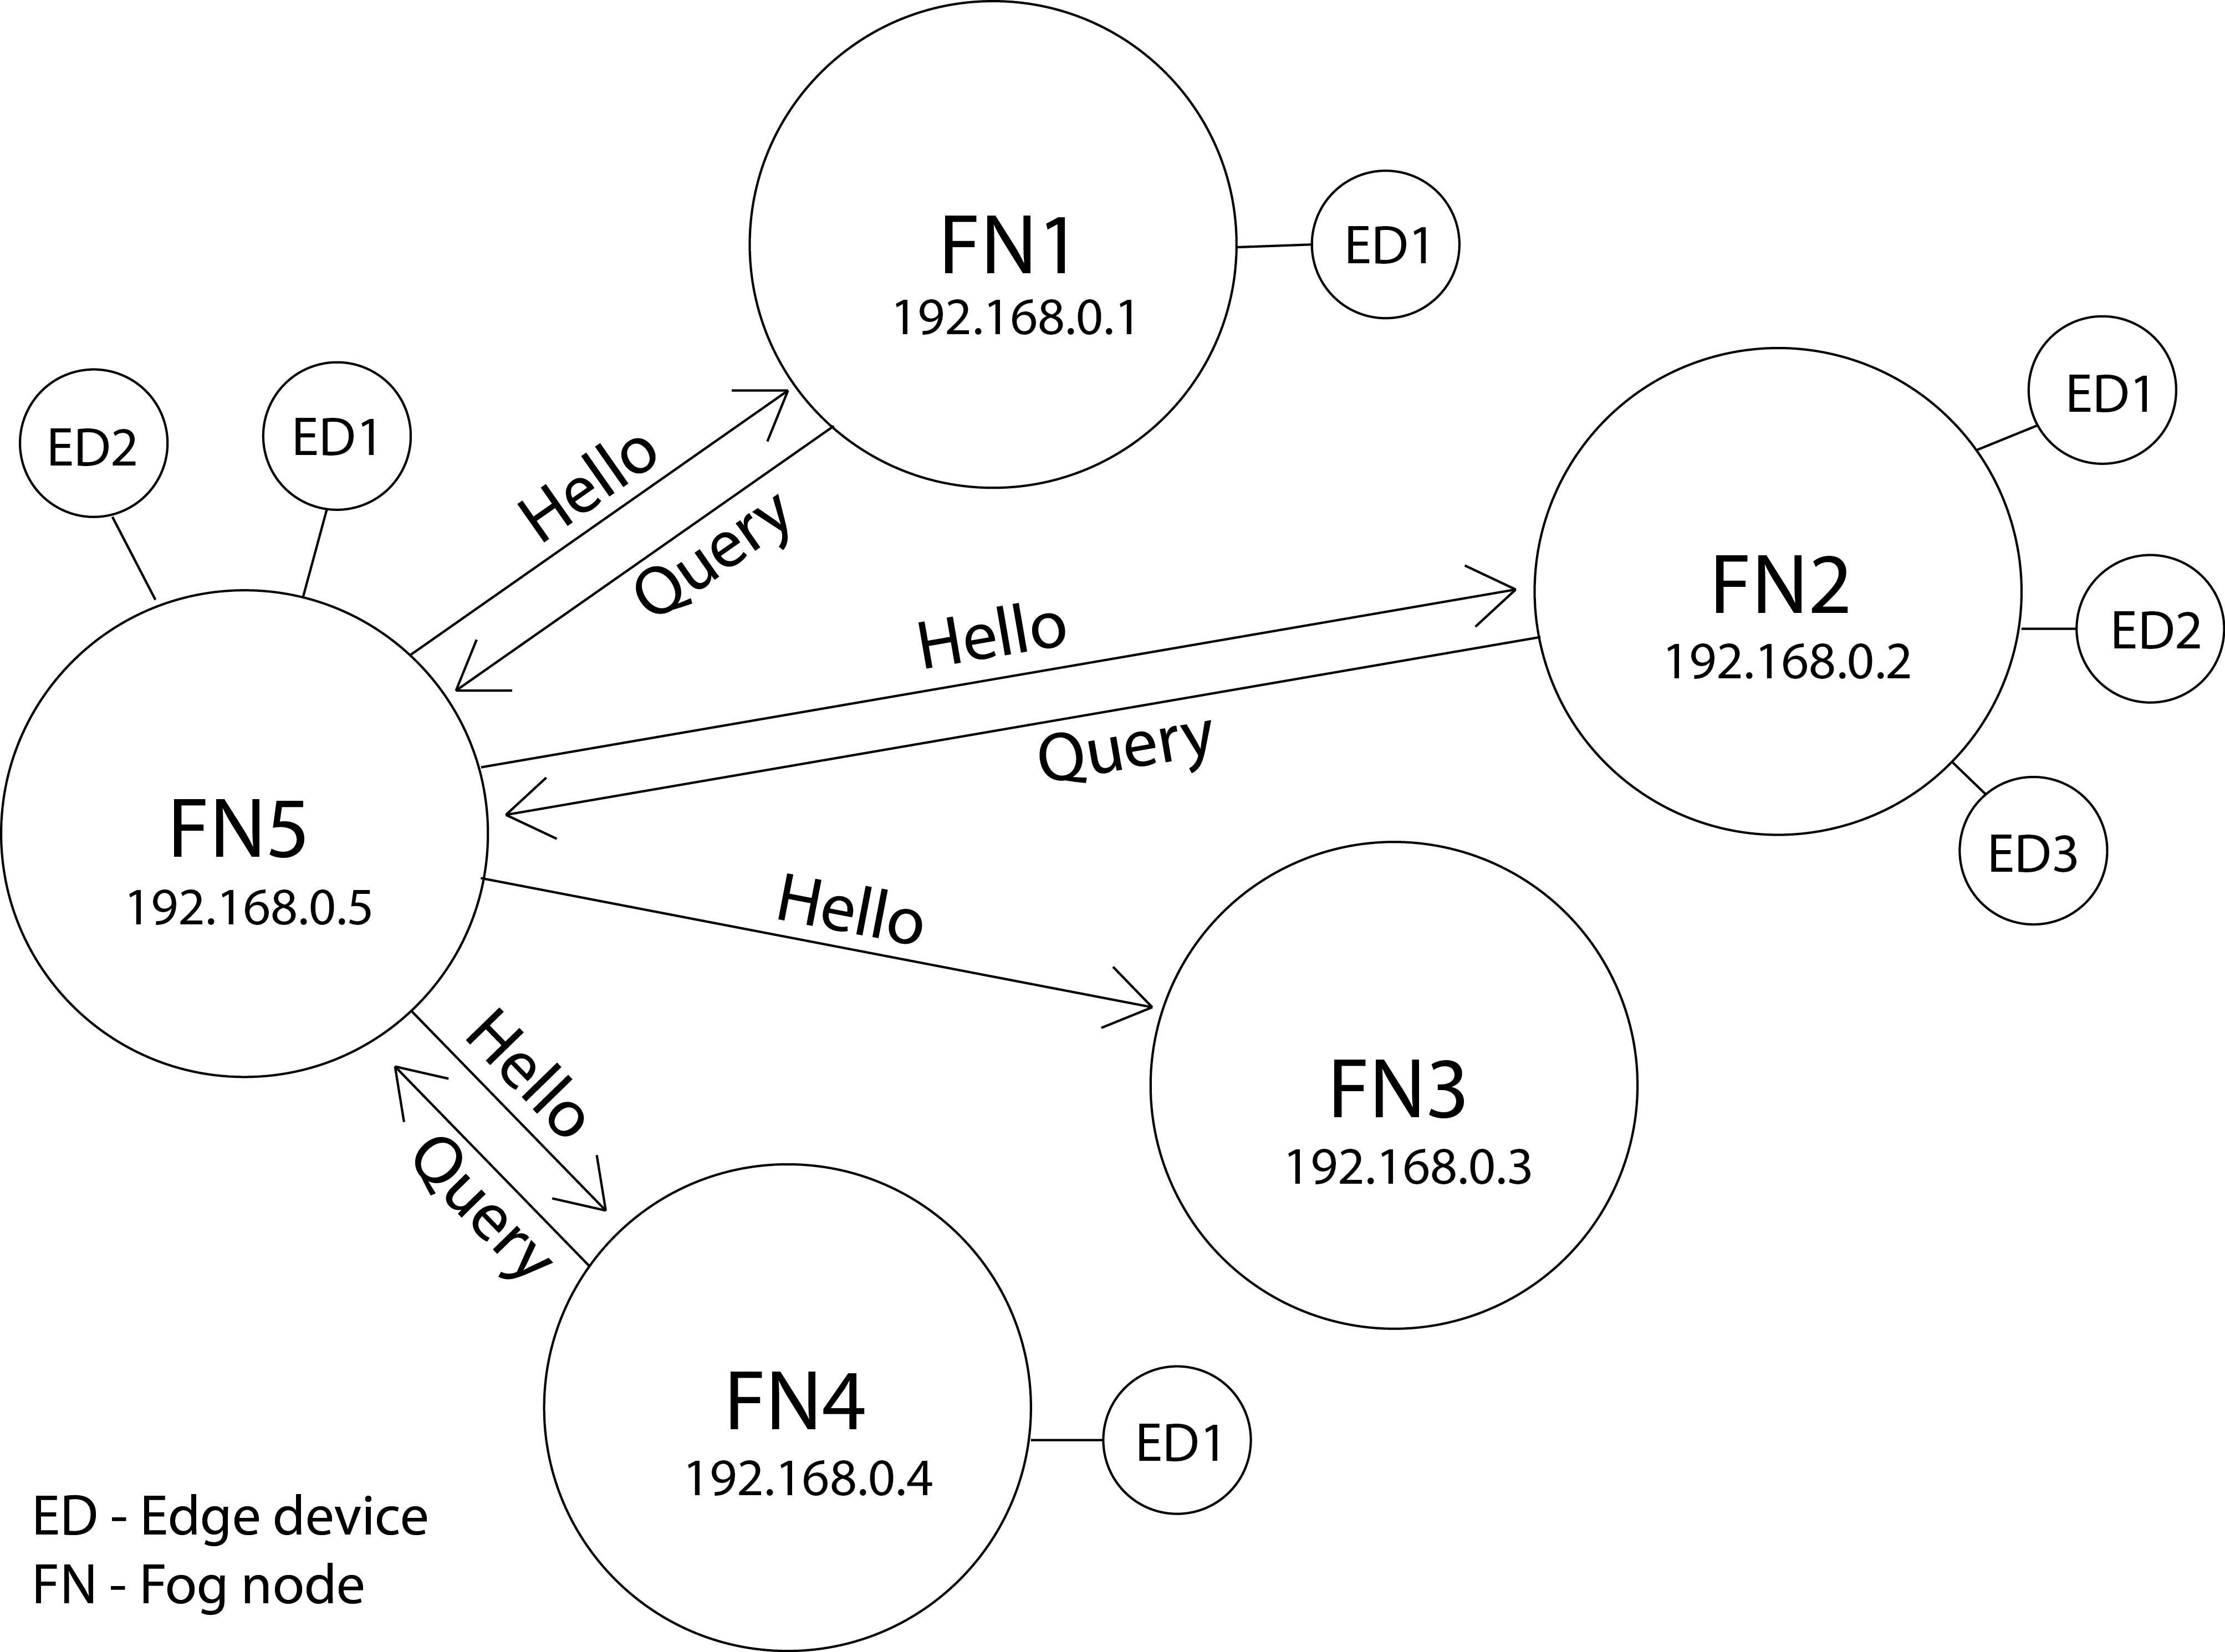
\includegraphics[width=.8\textwidth]{fig6.png}
    \caption [Requisição entre fog nodes]
    {\label{fig:fig6} Requisição entre fog nodes.}
\end{figure}


\subsection{Gerenciamento de recursos}

A manutenibilidade da lista de recursos globais é relevante para que o protocolo funcione de acordo com a especificação, pois, a névoa deverá saber quando um nodo, ou recurso dele, deixou de fazer parte da rede.
Para tal, faz-se necessário a utilização de alguns mecanismos de controle.
Esses controles são realizados em duas esferas, a primeira trata da inserção ou remoção de um nodo na rede,
já a segunda refere-se a inserção ou remoção de um edge device vinculado a um nodo qualquer.


Inicialmente abordaremos a entrada e saída de nodos da névoa, e para esta subseção será utilizado o cenário da Figura \ref{fig:fig6} quando necessário.
O Pseudocódigo \ref{alg:alg1} demonstra, de forma sucinta, a política de atualização que cada nodo deverá implementar no recebimento de mensagens de keep alive.


\begin{algorithm}[H]
    \begin{center}
        \begin{algorithmic}[1]
            \STATE \textbf{function} $\text{Policy(ip, epoch, myEpoch)}$
            \STATE \hspace{\algorithmicindent} \textbf{if} $\text{exists(ip)}$
            \STATE \hspace{\algorithmicindent} \hspace{\algorithmicindent} \textbf{if} $\text{epochHasChanged(epoch, myEpoch)};$
            \STATE \hspace{\algorithmicindent} \hspace{\algorithmicindent} \hspace{\algorithmicindent} $\text{resources = getResourcesCoAP(ip, '/.well-known/core')};$
            \STATE \hspace{\algorithmicindent} \hspace{\algorithmicindent} \hspace{\algorithmicindent} $\text{update(ip, resources)};$
            \STATE \hspace{\algorithmicindent} \textbf{else}
            \STATE \hspace{\algorithmicindent} \hspace{\algorithmicindent} $\text{resources = getResourcesCoAP(ip, '/.well-known/core')};$
            \STATE \hspace{\algorithmicindent} \hspace{\algorithmicindent} $\text{insert(ip, resources)};$
            \STATE \hspace{\algorithmicindent} $\text{sendAcknowledgement(ip)};$

        \end{algorithmic}
    \end{center}
    \caption[Política de atualização de recursos]%
        {\label{alg:alg1} Política de atualização de recursos.}%
    \end{algorithm}

No momento em que o nodo recebe a resposta da chamada de função \textit{getResourcesCoAP}, contendo os recursos providos pelo nodo requisitado, aquele deverá armazenar as informações em uma estrutura de dados adequada.
Essa estrutura de dados estará implementada em todos os nodos da névoa, e a partir dela será possível realizar o gerenciamento dos recursos de forma simples e eficiente.
O trecho abaixo define, por ora, o formato dos dados que serão utilizados em cada nodo.


\begin{verbatim}
    Fog = {
        string ip;
        string resources[];    
    };
    Fog fogs[];
    string myResources[];
\end{verbatim}

De posse da Figura \ref{fig:fig6} como cenário, do algoritmo de atualização \ref{alg:alg1}, e da estrutura de dados previamente descrita,
demonstramos abaixo o estado em que se encontram os dados armazenados em FN2 após a aplicação do método.

\begin{verbatim}
    fogs: [
        {
            ip: '192.168.0.1',
            resources: [ 'ED1' ]
        },
        {
            ip: '192.168.0.3',
            resources: [ ]
        },
        {
            ip: '192.168.0.4',
            resources: [ 'ED1' ]
        },
        {
            ip: '192.168.0.5',
            resources: [ 'ED1', 'ED2' ]
        }
    ];
    myResources: [ 'ED1', 'ED2', 'ED3' ];
\end{verbatim}

Visto isso, é imprescindível que os nodos mantenham seus dados consistentes, pois, após adicionar o novo nodo em sua lista de fogs, o protocolo precisa ser capaz de perceber quando um elemento
deixou de fazer parte do processo. Assim, a manutenção dos estados será abordado de forma similar as mensagens de \textit{keep alive} utilizadas no protocolo BGP\cite{Rekhter:1995}.
Mensagens de keep alive são adotadas para que os nodos da rede avisem seus vizinhos que ainda estão em operação, pois, sem esse procedimento seria difícil
saber quando remover um IP da lista de recursos. Portanto, para manter a lista atualizada, este protocolo implementa mensagens desse tipo.

As mensagens de keep alive serão transmitidas sob multicast em um intervalo de trinta segundos, porém, este é apenas um valor arbitrário, e pode ser alterado
para que a solução obtenha uma melhor eficiência.
Após o recebimento da mensagem de keep alive, os nodos deverão respondê-las indicando que ainda estão em operação.
Caso o nodo não responda a mensagem de keep alive, este será marcado como parcialmente inativo pelo remetente da mensagem.
Quando o nodo solicitante realizar outra mensagem de keep alive e o nodo que já estava marcado com parcialmente inativo não responder, o mesmo será removido da lista de recursos do
solicitante, e assim é possível saber quando um nodo deixou de fazer parte da névoa.
Para realizar este controle será preciso adicionar na estrutura \textit{Fog} a propriedade boleana, denominada \textit{isReplyingKeepAlive}, que indica se o nodo está respondendo a solicitações de keep alive.

As mensagens de keep alive mantém os nodos informados sobre o estado de seus vizinhos, mas não conseguem indicar informações relacionadas aos edge device.
Consequentemente, não é possível saber quando um edge device parou ou iniciou sua operação em um nodo ativo.

Para que seja possível detectar esse tipo de comportamento, o protocolo proposto deverá implementar a técnica denominada \textit{época},
e servirá para que os nodos mantenham ciênia sobre o estado dos edge devices de seus vizinhos de rede.
Para isso, uma nova propriedade denominada \textit{epoch}, do tipo inteiro, deverá ser adicionada a estrutura de dados, e estará presente tanto no nodo em si quanto em cada item da lista de fogs.
O valor da \textit{epoch} será incrementado em uma unidadade a toda alteração observada no nodo, seja pelo acréscimo ou pela remoção de edge devices.

Esta observação atuará realizando requisições para a URI /.well-known/core no endereço de loopback do próprio nodo,
assim, obterá seus recursos disponíveis e poderá comparar com os que possui armazenado em sua estrutura de dados.
Havendo divergências, como mencionado anteriormente, a propriedade época será incrementada em uma unidadade.

A partir de agora, então, todas as mensagens de keep alive deverão conter a época do nodo que está realizando o multicast.
Assim, todo nodo que receber a mensagem poderá comparar a época recebida na mensagem com a época que possui armazenada em sua lista de fogs referente ao remetente da mensagen.
Havendo divergência de épocas, este deverá realizar uma nova requisição para atualizar sua lista de recursos referente aquele nodo em específico.

Após as alterações realizadas na estrutura de dados, abaixo temos o novo modelo que suportará as funcionalidades propostas.
\begin{verbatim}
    Fog = {
        string ip;
        string resources[];
        int epoch;
        boolean isReplyingKeepAlive;
    }
    Fog fogs[];
    string myResources[];
    int epoch;
\end{verbatim}